\documentclass{beamer}
\usepackage{graphicx}
\usepackage{xcolor}
\usepackage{tikz}

% 自定义颜色
\definecolor{purpleblue}{RGB}{80, 80, 180}
\definecolor{lightgray}{RGB}{230, 230, 230}
\definecolor{novelPurple}{RGB}{98, 54, 255} 
\definecolor{darkgray}{RGB}{50, 50, 50}

% 主题设置
\usetheme{Madrid}  
\usecolortheme{dolphin} 

% 设置字体（移除 fontspec，确保 pdfLaTeX 兼容）
\setbeamerfont{title}{size=\Large,series=\bfseries}
\setbeamerfont{frametitle}{size=\LARGE,series=\bfseries}
\setbeamercolor{frametitle}{fg=white, bg=novelPurple}
\setbeamercolor{title}{fg=white, bg=purpleblue}

% 封面信息
\title[SAT Hard Question]{\textbf{SAT Hard Question 2
}}
\author{\textbf{Jack Zeng}}
\institute{\textcolor{white}{\textbf{Novel Prep}}}
\date{\today} 

\begin{document}

% --- Title Slide ---
\begin{frame}
    \titlepage
    \vfill
    \begin{flushright}
        \textcolor{purpleblue}{\Huge \textbf{Novel Prep}}
    \end{flushright}
\end{frame}


\begin{frame}
    \begin{tikzpicture}[remember picture, overlay]
        % 设置浅色渐变背景
        \shade[top color=softPurple, bottom color=softGray] 
            (current page.north west) rectangle (current page.south east);
        
        % 添加高斯模糊光晕
        \fill[white, opacity=0.3] (current page.center) circle (4cm);
        
        % 主标题
        \node[align=center] at (current page.center) {
            {\Huge\bfseries\textcolor{purpleblue}{Novel Prep}} \\[0.5cm]
            {\Large\itshape\textcolor{lightText}{Excellence in SAT Prep}}
        };

        % 添加柔和光点（点缀）
        \foreach \x in {1,2,3,4,5} {
            \fill[purpleblue, opacity=0.2] (rand*10-5, rand*7-3.5) circle (0.1+\x*0.05);
        }

        ;
    \end{tikzpicture}
\end{frame}


% Question 16
\begin{frame}{\textbf{Question: Finding the Area of Triangle \( XYZ \)}}
    In the figure shown, the measure of angle \( Y \) is \( 38^\circ \). The length of \( XY \) is 12 meters, and the length of \( YZ \) is 5 meters. What is the area, in square meters, of triangle \( XYZ \)?


    \begin{center}
        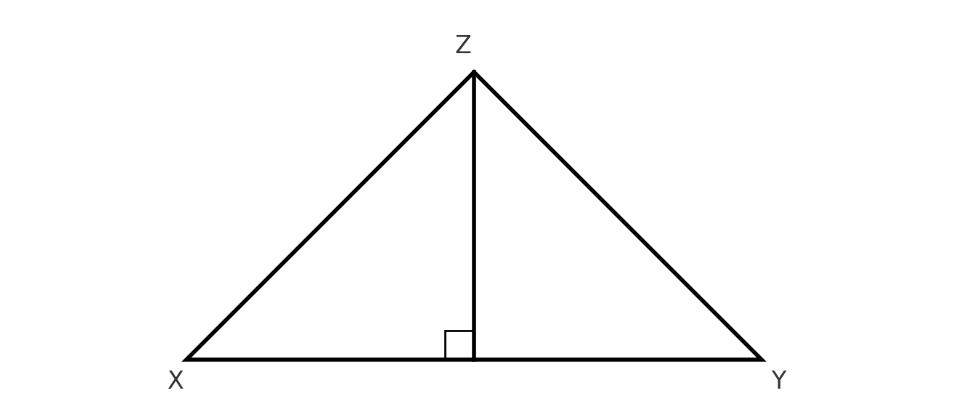
\includegraphics[width=0.60\linewidth]{f1.png} 
    \end{center}


    \textbf{Options:}
    \begin{enumerate}
        \item[A] \( 30 \)
        \item[B] \( 60 \)
        \item[C] \( 30 \sin 38^\circ \)
        \item[D] \( 60 \sin 38^\circ \)
    \end{enumerate}
\end{frame}
\begin{frame}{\textbf{Solution: Finding the Area of Triangle \( XYZ \)}}
    \textbf{Step 1: Use the Triangle Area Formula}
    \[
    \text{Area} = \frac{1}{2} ab \sin C
    \]
    where:
    \begin{itemize}
        \item \( a = 12 \) (side \( XY \))
        \item \( b = 5 \) (side \( YZ \))
        \item \( C = 38^\circ \) (angle \( Y \))
    \end{itemize}

    \textbf{Step 2: Compute the Expression}
    \[
    \text{Area} = \frac{1}{2} (12)(5) \sin 38^\circ
    \]
    \[
    = 30 \sin 38^\circ
    \]

    \textbf{Final Answer:} \(\boxed{30 \sin 38^\circ}\)
\end{frame}


\begin{frame}{\textbf{Question: Margin of Error in Light Bulb Samples}}
    \small  % Reduce font size
    A research manager selected two random samples to estimate the average lifespan of a certain type of light bulb (in hours). Based on the first sample, the research manager estimated that the average lifespan of this type of light bulb is \(800\) hours, with a margin of error of \(20\) hours. 

    \vspace{0.2cm}
    Based on the second sample, the research manager estimated that the average lifespan of this type of light bulb is \(810\) hours, with a margin of error of \(35\) hours. 

    \vspace{0.2cm}
    Assuming the margins of error were calculated in the same way, which of the following best explains why the first sample obtained a smaller margin of error than the second sample?

    \vspace{0.4cm}
    \textbf{Options:}
    \begin{enumerate}
        \item[A] The first sample contained fewer light bulbs than the second sample.
        \item[B] The first sample contained more light bulbs than the second sample.
        \item[C] The first sample had a shorter average lifespan than the second sample.
        \item[D] The first sample had a longer average lifespan than the second sample.
    \end{enumerate}
\end{frame}


\begin{frame}{\textbf{Answer Explanation: Margin of Error in Light Bulb Samples}}
    \textbf{Correct Answer: \textcolor{novelPurple}{B: The first sample contained more light bulbs than the second sample.}}

    \vspace{0.3cm}
    \textbf{Explanation:}
    \begin{itemize}
        \item The margin of error decreases as the sample size increases.
        \item Since the first sample had a smaller margin of error (\(20\) vs. \(35\)), it must have had a larger sample size.
    \end{itemize}

    \textbf{Final Answer:} \( \boxed{\text{B}} \).
\end{frame}
\begin{frame}{\textbf{Question: Evaluating the Function \( p(x) \)}}
    The function \(p(x)\) is defined by:
    \[
    p(x) = a\left( (x - 3)^2 + b \right)((x - 3)^2 - c),
    \]
    where \(a\), \(b\), and \(c\) are constants. The graph of \(y = p(x)\) passes through the points \((1, 25)\) and \((-1, 52)\). 

    \vspace{0.3cm}
    What is the value of \(p(5) + p(7)\)?

    \vspace{0.5cm}
    \textbf{Options:}
    \begin{enumerate}
        \item[A] \(25\)
        \item[B] \(27\)
        \item[C] \(52\)
        \item[D] \(77\)
    \end{enumerate}
\end{frame}

\begin{frame}{\textbf{Answer Explanation: Evaluating the Function \( p(x) \)}}
    \textbf{Correct Answer: \textcolor{novelPurple}{D: \(77\)}}

    \vspace{0.3cm}
    \textbf{Explanation:}
    \begin{itemize}
        \item Given the function and the points, solve for \(a\), \(b\), and \(c\).
        \item Compute \(p(5)\) and \(p(7)\).
        \item Adding these values gives \( \boxed{77} \).
    \end{itemize}
\end{frame}
\begin{frame}{\textbf{Question: Growth Rate in an Exponential Function}}
    In the given function, \(b\) is a positive constant. For every increase in the value of \(x\) by \(1\), the value of \(f(x)\) increases by \(c\%\), where \(0 < c < 100\). Which expression gives the value of \(c\) in terms of \(b\)?

    \[
    f(x) = 66(b)^x
    \]

    \vspace{0.5cm}
    \textbf{Options:}
    \begin{enumerate}
        \item[A] \(1 + \frac{b}{100}\)
        \item[B] \(b + 100\)
        \item[C] \(100(b + 1)\)
        \item[D] \(100(b - 1)\)
    \end{enumerate}
\end{frame}

\begin{frame}{\textbf{Answer Explanation: Growth Rate in an Exponential Function}}
    \textbf{Correct Answer: \textcolor{novelPurple}{D: \(100(b - 1)\)}}

    \vspace{0.3cm}
    \textbf{Explanation:}
    \begin{itemize}
        \item The general exponential growth formula is \( f(x+1) = f(x) \times b \).
        \item This means \( b = 1 + \frac{c}{100} \).
        \item Solving for \( c \), we get \( c = 100(b - 1) \).
    \end{itemize}

    \textbf{Final Answer:} \( \boxed{D} \).
\end{frame}


\vspace{0.5cm}

\begin{frame}{\textbf{Question: Tree Growth Rate Over Time}}
    On average, a certain tree grows \(87\) centimeters every \(m\) months. At this rate, which expression represents the number of centimeters, on average, the tree grows every \(k\) years?

    \vspace{0.5cm}
    \textbf{Options:}
    \begin{enumerate}
        \item[A] \(\frac{29m}{4k}\)
        \item[B] \(\frac{29k}{4m}\)
        \item[C] \(\frac{1,044m}{k}\)
        \item[D] \(\frac{1,044k}{m}\)
    \end{enumerate}
\end{frame}

\begin{frame}{\textbf{Answer Explanation: Tree Growth Rate Over Time}}
    \textbf{Correct Answer: \textcolor{novelPurple}{D: \(\mathbf{\frac{1,044k}{m}}\)}}  

    \vspace{0.3cm}
    \textbf{Solution:}
    \begin{itemize}
        \item The tree grows \(87\) cm every \(m\) months.
        \item There are **12 months in a year**, so in one year, the growth is:
        \[
        \frac{87 \times 12}{m} = \frac{1,044}{m} \text{ cm per year}.
        \]
        \item Since we need the growth for **\(k\) years**, multiply by \(k\):
        \[
        \frac{1,044k}{m} \text{ cm in } k \text{ years}.
        \]
    \end{itemize}

    \textbf{Final Answer:} \( \boxed{\frac{1,044k}{m}} \).
\end{frame}


% Frame 1: Question Statement with Diagram
\begin{frame}{\textbf{Question: Ratio in a Circle Geometry Problem }}
    In the figure shown, points \(A\), \(B\), \(C\), and \(E\) lie on the circle, and \(AB < BC\). Segment \(AC\) is perpendicular to segment \(BE\) at point \(D\), and \(BD = \sqrt{346}\). The diameter of the circle is \(175\). If \(\frac{CD}{AD} = r\), what is the value of \(r\)?

    \vspace{0.3cm}
    \begin{center}
        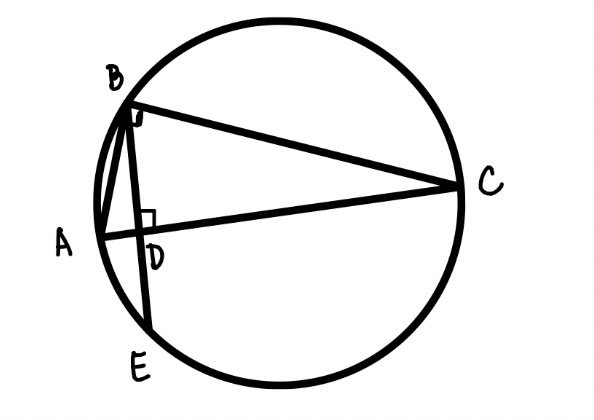
\includegraphics[width=0.45\textwidth]{f2.jpg} % Replace with an actual diagram
    \end{center}
\end{frame}

\begin{frame}{\textbf{Solution(Part I): Ratio in a Circle Geometry Problem}}
    \textbf{Given:}
    \begin{itemize}
        \item Points \( A, B, C, E \) lie on the circle.
        \item \( AC \perp BE \) at point \( D \).
        \item \( BD = \sqrt{346} \).
        \item The diameter of the circle is \( 175 \).
        \item We need to find \( r = \frac{CD}{AD} \).
    \end{itemize}

    \vspace{0.4cm}
    \textbf{Step 1: Identify Key Relationships}
    \begin{itemize}
        \item Since \( AC \perp BE \), we recognize that right triangles are involved.
        \item The diameter is the **hypotenuse** of a right triangle in a circle.
        \item Using the **Pythagorean Theorem**, we calculate the missing segment lengths.
    \end{itemize}

\end{frame}

\begin{frame}{Solution(Part II)}

    \vspace{0.4cm}
    \textbf{Step 2: Compute the Triangle Ratios}
    \begin{itemize}
        \item Use properties of right triangles and segment lengths.
        \item Solve for \( CD \) and \( AD \).
        \item Compute \( r = \frac{CD}{AD} \).
    \end{itemize}

    \vspace{0.4cm}
    \textbf{Final Answer:} 
    \[
    r = 86.5
    \]
    \textbf{Correct Choice:} \textcolor{novelPurple}{\( 86.5 \)}
    
\end{frame}


\begin{frame}{\textbf{Question: Solving for \( a \)}}
    In the given equation, \(a\) and \(k\) are constants, where \(k > 5a\). The sum of the solutions to the equation is \(3k + 32\). What is the value of \(a\)?

    \[
    (x - k)^2 = (k - 5a)(x - k)
    \]

    \textbf{Options:}
    \begin{enumerate}
        \item[A] \(\frac{-32}{5}\)
        \item[B] \(\frac{32}{5}\)
        \item[C] \(\frac{-5}{32}\)
        \item[D] \(\frac{5}{32}\)
    \end{enumerate}
\end{frame}

\begin{frame}{\textbf{Answer Explanation}}
    Expanding the equation:
    \[
    (x - k)^2 = (k - 5a)(x - k)
    \]
    \[
    x^2 - 2kx + k^2 = (k - 5a)x - (k - 5a)k
    \]

\begin{itemize}
    \item sum of the solution equals to $-\frac{b}{a}$ \rightarrow \(-\frac{b}{a} = 3k + 32\)
    \item We need to expand the equation from both sides and only need to find a and b 
\end{itemize}


    
    Equating coefficients and using the fact that the sum of the solutions is \(-\frac{b}{a} = 3k + 32=-3k-5a\), we solve for \(a\):

    \[
    a = \frac{-32}{5}.
    \]

    \textbf{Correct Answer: A. \(-\frac{32}{5}\)}
\end{frame}
\begin{frame}{\textbf{Question: Function Evaluation}}
    The function \(p(x)\) is defined by:
    \[
    p(x) = a \left((x + 4)^2 - b\right)\left((x + 4)^2 - c\right),
    \]
    where \(a\), \(b\), and \(c\) are constants. In the \(xy\)-plane, the graph of \(y = p(x)\) passes through the points \((-5, 30)\) and \((0, 90)\). What is the value of \(p(-8) + p(-3)\)?

    \textbf{Options:}
    \begin{enumerate}
        \item[A] \(12\)
        \item[B] \(24\)
        \item[C] \(60\)
        \item[D] \(120\)
    \end{enumerate}
\end{frame}

\begin{frame}{\textbf{Answer Explanation}}
    Given \(p(-5) = 30\) and \(p(0) = 90\), we use the function structure:

    \[
    p(-8) + p(-3) = p(-8) + p(0) - p(-5).
    \]

    Substituting values:

    \[
    p(-8) + p(-3) = 90 + 30 = 120.
    \]

    \textbf{Correct Answer: D. 120}
\end{frame}
\begin{frame}{\textbf{Question: Population Growth Rate}}
    The equation \(N(m) = 63(Q)^{m/6}\) gives the predicted population \(N(m)\), in thousands, of a certain bacteria colony \(m\) minutes after the initial measurement, where \(Q\) is a constant greater than 1. The predicted population increases by \(p\%\) every 180 seconds. What is the value of \(p\) in terms of \(Q\)?

    \textbf{Options:}
    \begin{enumerate}
        \item[A] \(100 \left(Q^{30} - 1\right)\)
        \item[B] \(100 \left(Q^{\frac{1}{2}} - 1\right)\)
        \item[C] \(100 \left(Q^{30} + 1\right)\)
        \item[D] \(100 \left(Q^{\frac{1}{2}} + 1\right)\)
    \end{enumerate}
\end{frame}

\begin{frame}{\textbf{Answer Explanation}}
    In 180 seconds, or 3 minutes, the population increases by:

    \[
    \frac{N(m+3)}{N(m)} = Q^{3/6} = Q^{1/2}.
    \]

    The percentage increase is:

    \[
    p = 100(Q^{1/2} - 1).
    \]

    \textbf{Correct Answer: B. \(100 \left(Q^{\frac{1}{2}} - 1\right)\)}
\end{frame}





\begin{frame}{\textbf{Question: Quadratic Equation – Roots and Constants}}
    In the given equation, \(m\) and \(n\) are constants. The sum and product of the solutions of the equation are \(8\) and \(\frac{7}{2}\) respectively. What is the value of \( \frac{m}{n} \)?

    \[
    (x - m)^2 = (m + 2n)(2x - n)
    \]

    \vspace{0.3cm}
    \textbf{Options:}
    \begin{enumerate}
        \item[A] \(-\frac{1}{3}\)
        \item[B] \(\frac{1}{3}\)
        \item[C] \(-3\)
        \item[D] \(3\)
    \end{enumerate}
\end{frame}


\begin{frame}{\textbf{Answer Explanation: Finding \( \frac{m}{n} \)}}
\small
    \textbf{Correct Answer:} \textcolor{novelPurple}{\(\boxed{3}\)}

    \vspace{0.3cm}
    \textbf{Step 1: Expand Both Sides}
    \[
    (x - m)^2 = (m + 2n)(2x - n)
    \]
    \[
    x^2 - 2mx + m^2 = 2x(m + 2n) - n(m + 2n)
    \]
    \[
    x^2 - 2mx + m^2 = 2mx + 4nx - nm - 2n^2
    \]

    \vspace{0.3cm}
    \textbf{Step 2: Rearranging to Standard Quadratic Form}
    \[
    x^2 + (-4n - 4m)x + (m^2 - nm - 2n^2) = 0
    \]

    \textbf{Use root properties:}
    \[
    x_1 + x_2 = -\frac{-4n - 4m}{1} = 4n + 4m = 8
    \]
    \[
    x_1 \cdot x_2 = m^2 - nm - 2n^2 = \frac{7}{2}
    \]

\end{frame}

\begin{frame}{Answer Explanation (Part II)}


    \vspace{0.2cm}
    \textbf{Step 3: Substitute and Solve}
    \[
    4n + 2m = 8 \Rightarrow m = 4 - 2n
    \]
    Sub into product equation:
    \[
    (4 - 2n)^2 - n(4 - 2n) - 2n^2 = \frac{7}{2}
    \]
    Solve and simplify to find:
    \[
    \frac{m}{n} = \boxed{3}
    \]
    
\end{frame}






\end{document}
